\documentclass{scrartcl}
\usepackage{etex}
\usepackage{german}
\usepackage{pst-all}
\usepackage[utf8]{inputenc} 

\usepackage[arrow, matrix, curve]{xy}

\usepackage{amsmath,amsthm,amssymb}

\usepackage{tikz}
\usepackage{wrapfig}

\title{Insel der Zahlen}
\author{Ali und Rachid}
\date{die Epoche}

\pdfinfo{
   /Author (Max Mustermann)
   /Title  (Insel der Zahlen)
   /Subject (Insel der Zahlen Subject)
   /Keywords (Sandkasten;Zahlen;Insel)
}

\begin{document}
%% Titel und Inhaltsverzeichnis des Artikels hier
%% ausgeben

\maketitle

\begin{align}
a&=b
\end{align}

Klappt das? Auch \LaTeX{}? Anscheined ja. :-) , oder nicht?

Scheiße, alle Formatierungsbefehle vergessen :-(
\newline
Wie ging das nochmal mit 'ner Gleichung?

Warum darf ich denn in einer displaymath-Umgebung keine Leerzeilen haben? ein Bug?

Aus l2kurz.tex (z.B. vom Dante-Server):

\begin{displaymath}
\sum_{i=1}^{n} \qquad
\int_{0}^{\frac{\pi}{2}} \qquad
\int \limits_{-\infty}^{+\infty}\\
\end{displaymath}

\begin{displaymath}
\textrm{Ok, meine Stunde}\ldots \varnothing \texttt{:-)} \qquad \  \qquad
\int \limits_{a}^{b} f(x) d x = F(b) - F(a)
\end{displaymath}

Gibt's denn im WS ein gleiches Projekt? Kollaborative Skipterstellung?? Eine sch"one Idee. Hat denn "uberhaupt jemand mitgearbeitet am Skript?

$ \varnothing $
BTW: Koma-Script rulez \texttt{:-)}

\begin{xy}
  \xymatrix{
      A \ar[r]^f \ar[d]_i    &   B \ar[d]^j  \\
      C \ar[r]_g             &   D   
  }
\end{xy}

SVN-Testtest

\begin{figure}
  \label{DFS-Bsp}
  \centering
  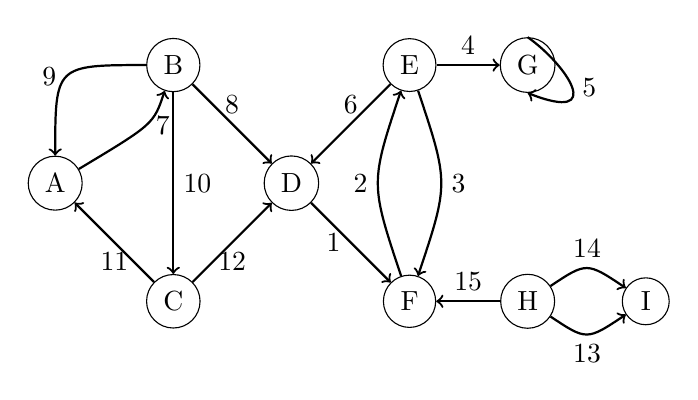
\begin{tikzpicture}
    
    \begin{scope}[shape=circle]
    \tikzstyle{every node}=[draw]
    \node (a) at (0, 0) {A};
    \node (b) at (1.5, 1.5) {B};
    \node (c) at (1.5, -1.5) {C};
    \node (d) at (3, 0) {D};
    \node (e) at (4.5, 1.5) {E};
    \node (f) at (4.5, -1.5) {F};
    \node (g) at (6, 1.5) {G};
    \node (h) at (6, -1.5) {H};
    \node (i) at (7.5, -1.5) {I};
    \end{scope}

  \begin{scope}[style=thick,->]
    \draw (d) -- (f) node[midway,left]{1};
    \draw (f) .. controls (4,0) .. (e) node[midway,left]{2};
    \draw (e) .. controls (5,0) .. (f) node[midway, right]{3};
    \draw (e) -- (g) node[midway, above]{4};
    \draw (g.north) .. controls (6.5, 1.5) and (7, 0.75) .. (g.south) node[midway, right]{5};
    \draw (e) -- (d) node[midway,above]{6};
    \draw (a) .. controls (1.25,0.75) .. (b) node[midway, right]{7};
    \draw (b) -- (d) node[midway, above]{8};
    \draw (b) .. controls (0,1.5) .. (a) node[midway, left]{9};
    \draw (b) -- (c) node[midway, right]{10};
    \draw (c) -- (a) node[midway, below]{11};
    \draw (c) -- (d) node[midway, below]{12};
    \draw (h) .. controls (6.75,-2) .. (i) node[midway, below]{13};
    \draw (h) .. controls (6.75,-1) .. (i) node[midway, above]{14};
    \draw (h) -- (f) node[midway,above]{15};
  \end{scope}

  \end{tikzpicture}
  \caption{Beispielgraph für Tiefensuche}
\end{figure}


\begin{wrapfigure}{r}{.2\textwidth}
  \begin{center}
    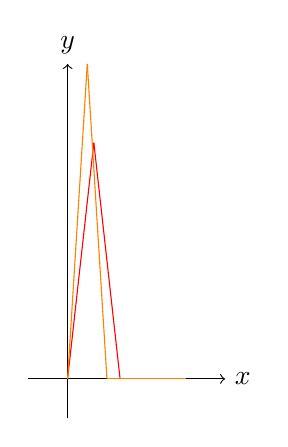
\begin{tikzpicture}
          \draw[->] (-0.5,0) -- (2,0) node[right] {$x$}; %
          \draw[->] (0,-0.5) -- (0,4) node[above] {$y$};%
          \draw [domain=0:1/3,red] plot (\x,3*3*\x);%
          \draw [domain=1/3:2/3,red] plot (\x,2*3-3*3*\x);%
          \draw [domain=2/3:1.5,red] plot (\x,0);%
 
          \draw [domain=0:1/4,orange] plot (\x,4*4*\x);%
          \draw [domain=1/4:2/4,orange] plot (\x,2*4-4*4*\x);%
          \draw [domain=2/4:1.5,orange] plot (\x,0);%
    \end{tikzpicture}
  \end{center}
\end{wrapfigure}
 
Lorem ipsum dolor sit amet, consectetur adipiscing elit. Duis congue dictum elit. Morbi ultricies laoreet massa, sed sagittis lorem laoreet et. Donec at erat non sem tristique rutrum vel vel justo. Vestibulum tincidunt pulvinar mi, a congue purus dignissim vel. Ut porttitor dignissim neque eget rutrum. Nunc gravida varius semper. Quisque et purus quam. Quisque ultricies tristique magna sit amet egestas. Mauris bibendum lacus semper justo consectetur blandit vitae non nisi. Etiam non augue nec est facilisis tempor. Nullam non diam vel erat fermentum gravida. Proin tincidunt turpis lobortis ante elementum suscipit. Curabitur congue, dolor fringilla feugiat blandit, quam libero euismod purus, eget commodo erat nibh a augue. Vestibulum ut tellus ac arcu semper facilisis.


\end{document}
